\section{Gitting started}	% huehue

\subsection{Repository aanmaken}
\frame{
	%\frametitle{Repository aanmaken}
	\begin{enumerate}
		\item Open terminal (windows: \alert{git-bash})
		\item \texttt{cd} naar map die je wil bijhouden
			(of \texttt{mkdir} een nieuwe)
		\item \texttt{git init}
		\item \texttt{git status}
	\end{enumerate}
	Als het goed is zie je nu \alert{niet}:
	\begin{center}
		{
			\small
			\texttt{fatal: Not a git repository or any of the parent directories: .git}
		}
	\end{center}
}

\subsection{Bestanden laten bijhouden}
\frame{
	\begin{enumerate}
		\item \texttt{git status}
		\item Bekijk 'untracked files'
		\item \texttt{git add bestand1 bestand2 map1}\\ of:
			\texttt{git add .}\\
			(map pakt alle bestanden erin mee, . is huidige map)
		\item \texttt{git commit -m "Eerste commit"}
	\end{enumerate}
	Resultaat: \texttt{(ja wat eigenlijk)}
}

\frame{
	\begin{center}
		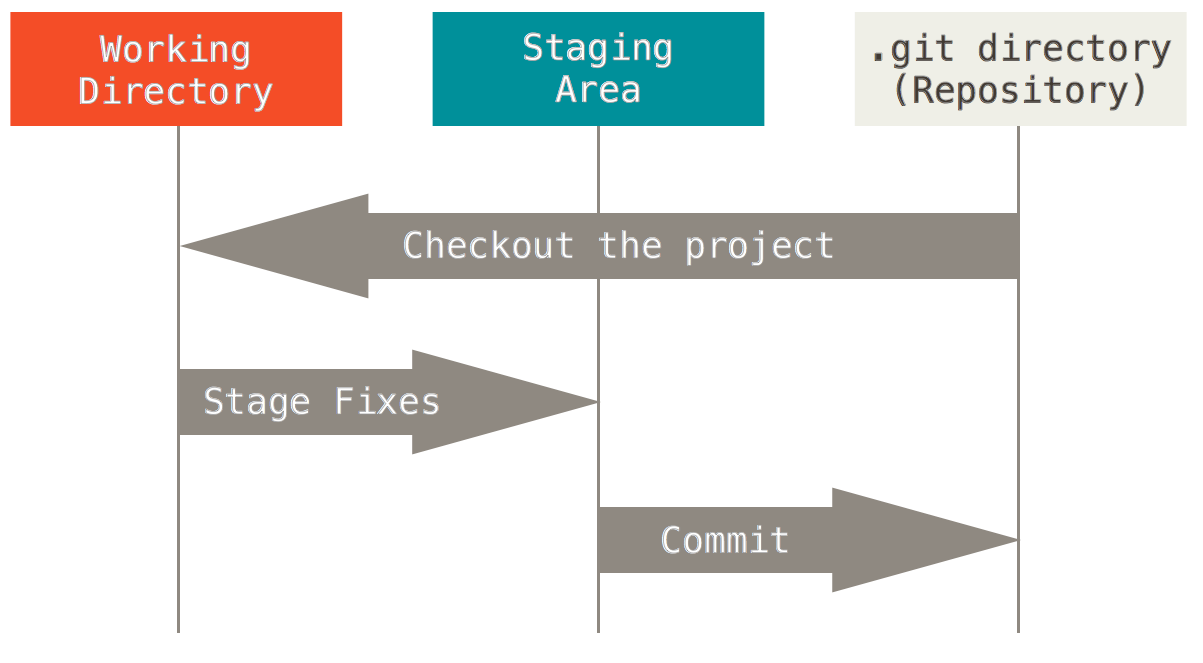
\includegraphics[width=\textwidth]{images/areas}
	\end{center}
}
